\chapter{bcg.h Documentation}
\ifsingle
\maketitle
\fi
\chaptermeta[2.0][2025-06-04]

\section{Introduction and Background}\label{sec:bcg-intro}
\textbf{bcg.h} file contains two functions: \textcolor{red}{\emph{tracer\_fluxes}} and \textcolor{red}{\emph{advection}} whose major purpose is to construct a solver for advective equation:
\begin{equation}
  \frac{\partial \Phi}{\partial t} + ( \mathbf{u} \cdot \nabla)\Phi = 0\label{equ:bcg-aim}
\end{equation}
where $\Phi$ is the scalar and $ \mathbf{u}$ is the velocity. The discrete time formulation of equation \ref{equ:bcg-aim} reads:
\begin{equation}
  \frac{\Phi^{n+1}-\Phi^{n}}{\Delta t} + \mathbf{A}^{n+\frac{1}{2}} = 0 \label{equ:bcg-general}
\end{equation}
Where $ \mathbf{A}^{n+ \frac{1}{2}}$ is the abbreviation of advection term. With the conservative constraints $\nabla \cdot \mathbf{u} = 0$, the integral form reads:
\begin{equation}
  \int_{\Gamma} A^{n+ \frac{1}{2}} = \int_{\Gamma} [( \mathbf{u}\cdot \nabla)\Phi]^{n+ \frac{1}{2}} = \int_{\Gamma} [\nabla\cdot( \mathbf{u} \Phi)]^{n+ \frac{1}{2}} = \int_{\partial \Gamma} ( \mathbf{u}^{n + \frac{1}{2}} \cdot \mathbf{n}) \Phi^{n+ \frac{1}{2}}
\end{equation}
where $ \mathbf{n}$ represents the normal direction of cell interface. For cartesian cell employed in Basilisk, the calculation turns out to be
\begin{equation}
  \Delta A^{n+ \frac{1}{2}} = \sum_{d} s_d u_{f,d}^{n+ \frac{1}{2}}\Phi_{f,d}^{n + \frac{1}{2}} 
\end{equation}
Note in this documentation, the subscript $f$ denotes face value stored in staggered mesh\cite{1965_Harlow}, otherwise it is cell-average value stored in center of the cell. Subscript $d$ is the notation of specific face ($e,w,n,s$ for 2D and $e,s,n,s,f,b$ for 3D) for a single cell. In addition, readers may found algebraic notation without $d$ such as $u_f$ in the upcoming discussion which refers to the same thing. This is because in the most cases $d$ is used to addressed spatial relationship between face and cell from cell-perspective, such relation shall vanish from face-perspective and so does $d$.

The following discussions are conducted under 2D condition and results of 3D is easily to obtain accordingly. $s_d$ represents sign function which reads
\begin{equation}
    s_d = 
    \left\{
    \begin{array}{cc}
    1\ \ d=e,n \\
    -1\ \ d=w,s
    \end{array}
    \right.
\end{equation}
The problem now becomes how to obtain $u_f^{n+1/2}$ and $\Phi_f^{n+1/2}$. Basilisk employs BCG scheme to tackle such issue. The scheme, which is originally named by three authors\cite{1989_Bell}, stems from the algorithm intending to apply second order Godunov method to incompressible flow. It obtains value at $n+\frac{1}{2}$ not by averaging but by considering the Taylor series, for each cell:
\begin{equation}
  \Tilde{\Phi}^{n+ \frac{1}{2}}_{f,d} = \Phi^n+ s_d\frac{\Delta}{2} \frac{\partial \Phi^n}{\partial x_d} + \frac{\Delta t}{2} \frac{\partial \Phi^n}{\partial t} + O(\Delta^2,\Delta t^2)
\end{equation}
Where $x_d=x$ for $d = e,w$ and $x_d=y$ for $d = n,s$. Replacing $ \frac{\partial \Phi^n}{\partial x_d}$ with Euler equation \ref{equ:bcg-aim} yielding 
\begin{equation}
  \Tilde{\Phi}^{n+ \frac{1}{2}}_{f,d} = \Phi^n + [s_d \frac{\Delta}{2}- \frac{\Delta t}{2} u_d] \frac{\partial \Phi^n}{\partial x_d} - \frac{\Delta t}{2} u_o \frac{\partial \Phi^n}{\partial x_o}\label{equ:bcg-taylor}
\end{equation}
where $u_d$ is the cell-centered value on $d$ direction (i.e. $u_x$ for $d = e,w$, $u_y$ for $d = n,s$). Subscript $o$ represents directions other than $d$.
Since aiming equation \ref{equ:bcg-aim} is advection-only, a simple upwind scheme is therefore employed\cite{2000_Martin,1998_Martin} to adapt each term in equation \ref{equ:bcg-taylor}:
\begin{align}
  \Tilde{\Phi}^{n+ \frac{1}{2}}_{f,d} &= \Phi^n + [s_d \frac{\Delta}{2}- max(\frac{\Delta t}{2} u_d,0)] \frac{\partial \Phi^n}{\partial x_d} - \frac{\Delta t}{2} u_o \overline{\frac{\partial \Phi^n}{\partial x_o}}\label{equ:bcg-upwind} \\
  \overline{\frac{\partial \Phi^n}{\partial x_o}} &= \left\{
  \begin{array}{cc}
       (\Phi^n[0] - \Phi^n[-1])/\Delta&\ if\ u_o>0 \\
       (\Phi^n[1] - \Phi^n[0])/\Delta&\ if\ u_o<0
  \end{array}
  \right.\label{equ:bcg-upwind2}
\end{align}
If not additionally declared, $\frac{\partial \Phi^n}{\partial x_d}$ is computed with central scheme.
Given four face values from each cell, each face now has two values from its neighbor cell which are left value and right value in traditional Godunov method. Unlike the traditional method which obtains the final face value $\Phi_{f,d}$ by solving Riemann problem, the upwind scheme is again applied to determine $\Phi_{f,d}$ in current algorithm (the value is counted from each face hence the subscript $d$ is omitted.)
\begin{equation}
    \Phi^{n+1/2}_{f}[0] = \left\{
    \begin{array}{cc}
         \Tilde{\Phi_f}[0]\ \ &u^{n+1/2}_f<0\\
         \Tilde{\Phi_f}[-1]\ \ &u^{n+1/2}_f>0\\
         \frac{1}{2}(\Tilde{\Phi_f}[0]+\Tilde{\Phi_f}[-1])\ \ &u^{n+1/2}_f=0
    \end{array}
    \right.
    \label{equ:bcg-upwindfinal}
\end{equation}
where $u_f$ is velocity on the same face and marker $[0],[-1]$ indicate the cell from which the face value is obtained. In mesh system of Basilisk, for face located at $(i-1/2,j)$ the $[0]$ (resp. $[-1]$) represents cell positioned at $(i,j)$ (resp. $(i-1,j)$). It is worth mentioning that the marker in current equation is associated with the direction. For example, if one calculates face value $\Phi_f^{n+1/2}$ on $x$ direction, the marker in equation \ref{equ:bcg-upwindfinal} indicates the relationship on $x$ direction while those in equation \ref{equ:bcg-upwind2} refers to relation on $y$ direction. Above discussion is the original algorithm on the paper, compensation is made in real code which shall be introduced in the following sections.

\section{Functions}

\subsection{\func{tracer\_fluxes}}
Given face velocity $u^{n+1/2}_f$, the face flux $u_{f}^{n+ \frac{1}{2}}\Phi_{f}^{n + \frac{1}{2}}$ is computed and stored on staggered mesh.
\subsubsection{Parameters}
\begin{center}
  \begin{tabular}{|c|c|c|c|c|}
    \hline
    Name & Data type & Status & Option/Default & Representation (before/after)\\[0.5ex]
    \hline\hline
    \para{f} & scalar & unchanged & compulsory & $\Phi^n$\\
    \hline
    \para{uf} & face vector & unchanged & compulsory & $u_f^{n+ \frac{1}{2}}$\\
    \hline
    \rowcolor{output} \para{flux} & face vector & \textbf{output} & compulsory & $u_f^{n+ \frac{1}{2}}\Phi_f^{n+\frac{1}{2}}$\\
    \hline
    \para{dt} & double & unchanged & compulsory & $\Delta t$\\
    \hline
    \para{src} & scalar & unchanged & compulsory & $ a^n$ \\
    \hline
  \end{tabular}
\end{center}

\subsubsection{Worth Mentioning Details}\label{sec:bcg-tracerdetail}
As discussed previously, specific face value on staggered mesh\cite{1965_Harlow} can be located by its spatial relation with corresponding cell. Take cell at $(i,j)$ as an example, figure \ref{fig:bcg-staggered} demonstrates notation of each face. Moreover such value can be iterated by calling macro $foreach\_face()$ in Basilisk. Thanks to this feature, the code can be constructed from face-perspective starting from equation \ref{equ:bcg-upwindfinal} rather than iterating every cell and compare two values for single faces.\par
Notably, different from original algorithm, two compensations are made in performing equation \ref{equ:bcg-upwindfinal} and equation \ref{equ:bcg-upwind} respectively. For the former one, the condition where $u_f^{n+1/2}=0$ merges into the second condition, the filter now reads:
\begin{equation}
    \Phi^{n+1/2}_{f}[0] = \left\{
    \begin{array}{cc}
         \Tilde{\Phi_f}[0]\ \ &u^{n+1/2}_f<0\\
         \Tilde{\Phi_f}[-1]\ \ &u^{n+1/2}_f\geq0
    \end{array}
    \right.
    \label{equ:bcg-upwindfinal2}
\end{equation}
For the latter one, $u_d$ is replaced by face value $u_f[]$ for simplicity in boundary condition settings. Consequently the upwind filter (i.e. the $max()$) is no longer needed in the second term of equation \ref{equ:bcg-upwind} since upwind scheme is automatically met owing to upwind selection originally conducted by equation \ref{equ:bcg-upwindfinal2}. 

\begin{figure}[H]
     \centering
     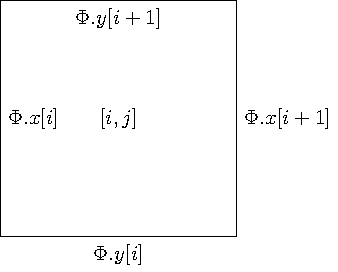
\includegraphics{image/bcg-h/staggered.pdf}
     \caption{Example of staggered mesh.}
     \label{fig:bcg-staggered}
\end{figure}
Given $u_f^{n+1/2}$, the procedure to compute face flux now becomes:
\begin{enumerate}
    \item Identify the upstream direction based on $u_f^{n+1/2}$.
    \item Choose corresponding cell to compute face flux based on equation \ref{equ:bcg-upwindfinal} and upstream direction obtained in previous step.
    \item According to equation \ref{equ:bcg-upwind} \ref{equ:bcg-upwind2}, add contribution from each direction and multiply the result by $u_f^{n+1/2}$ to obtain $u_f^{n+1/2}\Phi_f^{n+1/2}$.
\end{enumerate}
Yet another detail worth mentioning is the source term $a^n$ in current function. This is indeed preparation for solving non-Euler equation such as NS equation in 'centered.h'. Albeit compulsory here, such term is overall optional in the final function \func{advection} which shall be introduced in the upcoming section.

\begin{codesection}{subsubsection}{Program Workflow}
\codecomment{
  \textbf{Starting Point}\\
  \textbf{input}: \\
  \para{f} = $\Phi^n$ \para{uf} = $u_f^{n+ \frac{1}{2}}$\\ \para{flux}(empty) \para{dt}=$\Delta t$\\ \para{src} = $ \mathbf{g}^n$\\
  \textbf{gradient}:\\
  \para{g} = $\nabla$ \para{f} = $\nabla \Phi$
}

\begin{minted}{cpp}
void tracer_fluxes (scalar f,
		    face vector uf,
		    face vector flux,
		    double dt,
		    (const) scalar src)
{
  vector g[];
  gradients ({f}, {g});
\end{minted}

\codearrow

\codecomment{
  \textbf{Compute un}\footnote{A compensation is made here, see \ref{sec:bcg-tracerdetail} for detailed information}: \\
  \para{un}=$\frac{u_{f,d}^{n+1/2}\Delta t}{fm.x[i]\Delta}$\\
  \textbf{Identification of upstream direction}\\
  The notation of corresponding cell \para{i} is identified according to equation \ref{equ:bcg-upwindfinal2}.\\
  \para{s} = $s_d$\\
}

\begin{minted}{cpp}
  foreach_face() {
    double un = dt*uf.x[]/(fm.x[]*Delta + SEPS), s = sign(un);
    int i = -(s + 1.)/2.;
\end{minted}

\codearrow

\codecomment{
  \textbf{Contribution of Each Direction}\\
  \textbf{Main direction}\\
  \para{f2} = $\Phi^n[i] + \frac{\Delta}{2}[s_d- \frac{\Delta t}{\Delta}u_{f,d}^{n+1/2}] \frac{\partial \Phi^n}{\partial x_d}[i]$\\
  $+\frac{\Delta t}{2}\frac{a^n[-1]+a^n[0]}{2}$\\ 
  \textbf{Traversal direction}\\
  \textbf{compute $u_o$ in equation \ref{equ:bcg-upwind}}: \\
  \para{vn}(\para{wn})=$(u^{n+1/2}_{f,o}[i,0]+u^{n+1/2}_{f,o}[i,1])/(fm.e[i,0]+fm.e[i,1])$\\
  \textbf{component of other direction}:\\
  The gradient $\overline{\frac{\partial \Phi^n}{\partial x_o}}$ is first computed by upwind scheme based on direction of $u_o$ according to equation \ref{equ:bcg-upwind2}\\
  \para{fyy}(\para{fzz})= $\overline{\frac{\partial \Phi^n}{\partial x_o}}$\\
  \para{f2} -= $\frac{\Delta t}{2} u_o \overline{\frac{\partial \Phi^n}{\partial x_o}}$ 
}

\begin{minted}{cpp}
    double f2 = f[i] + (src[] + src[-1])*dt/4. + s*(1. - s*un)*g.x[i]*Delta/2.;
    #if dimension > 1
    if (fm.y[i] && fm.y[i,1]) {
      double vn = (uf.y[i] + uf.y[i,1])/(fm.y[i] + fm.y[i,1]);
      double fyy = vn < 0. ? f[i,1] - f[i] : f[i] - f[i,-1];
      f2 -= dt*vn*fyy/(2.*Delta);
    }
    #endif
    #if dimension > 2
    if (fm.z[i] && fm.z[i,0,1]) {
      double wn = (uf.z[i] + uf.z[i,0,1])/(fm.z[i] + fm.z[i,0,1]);
      double fzz = wn < 0. ? f[i,0,1] - f[i] : f[i] - f[i,0,-1];
      f2 -= dt*wn*fzz/(2.*Delta);
    }
    #endif
\end{minted}

\codearrow

\codecomment{
  \textbf{Assemble}\\
  assemble the final result, current direction is $d$\\
  \para{flux.d}=$u_{f,d}^{n+ \frac{1}{2}}\Phi_{f,d}^{n+ \frac{1}{2}}$\\
  after the $foreach\_face$ macro, the face flux on every face is obtained.
}

\begin{minted}{cpp}
    flux.x[] = f2*uf.x[];
  }
}
\end{minted}

\end{codesection}

\subsection{\func{advection}}
Given face flux $u^{n+1/2}_f\Phi^{n+1/2}_f$, compute $\Phi^{n+1} = \Phi^n-\Delta t A^{n+1/2}$.
\subsubsection{Parameters}
\begin{center}
  \begin{tabular}{|c|c|c|c|c|}
    \hline
    Name & Data type & Status & Option/Default & Representation (before/after)\\[0.5ex]
    \hline\hline
    \rowcolor{output} \para{tracers} & scalar* & update & compulsory & $\Phi^n$/ $\Phi^n-\Delta t A^{n+ \frac{1}{2}}$\\
    \hline
    \para{u} & face vector & unchanged & compulsory & $u_f^{n + \frac{1}{2}}$\\
    \hline
    \para{dt} & double & unchanged & compulsory & $\Delta t$\\
    \hline
    \para{src} & scalar* & unchanged & optional/NULL & $ \mathbf{g}^n$ \\
    \hline
  \end{tabular}
\end{center}

\subsubsection{Worth Mentioning Details}\label{sec:bcg-direction}
The data type $scalar*$ indicates the input can be vector, and each components will be treated as $scalar$ type data and are assembled into one $vector$ data eventually.\par
Given the face flux $u^{n+1/2}_f \Phi^{n+1/2}_f$, according to equation \ref{equ:bcg-aim}, for each cell the $\Phi^{n+1}$ yielding:
\begin{equation}
    \Phi^{n+1} = \Phi^n-\Delta t \sum_{d} s_d u_{f,d}^{n+ \frac{1}{2}}\Phi_{f,d}^{n + \frac{1}{2}}
\end{equation}
take $flux = u^{n+1/2}_f \Phi^{n+1/2}_f$ for cell located at $(i,j)$ the above equation reads
\begin{equation}
    \Phi^{n+1}[i,j] = \Phi^n[i,j] + \Delta t (flux.x[i] - flux.x[i+1] + flux.y[j] - flux.y[j+1])
\end{equation}

\begin{codesection}{subsubsection}{Program Workflow}
\codecomment{
  \textbf{Starting Point}\\
  \textbf{input}: \\
  \para{tracers} = $\Phi^n$ \para{u} = $u_f^{n+ \frac{1}{2}}$\\ \para{dt}=$\Delta t$ \para{src} = $ a^n$\\
}

\begin{minted}{cpp}
    struct Advection {
      scalar * tracers;
      face vector u;
      double dt;
      scalar * src; // optional
    };
    void advection (struct Advection p)
    {
      scalar * lsrc = p.src;
      if (!lsrc)
        for (scalar s in p.tracers)
          lsrc = list_append (lsrc, zeroc);
      assert (list_len(p.tracers) == list_len(lsrc));
\end{minted}

\codearrow

\codecomment{
  \textbf{Fluxes Compute}\\
  Traversal each elements in \para{tracers} (if \para{tracers} is vector, then this step traversal component on every direction)\\
  \textbf{computation}: \\
  \para{flux} = $\Phi_f^{n + \frac{1}{2}} u_f^{n + \frac{1}{2}}$\\
}

\begin{minted}{cpp}
  scalar f, src;
  for (f,src in p.tracers,lsrc) {
    face vector flux[];
    tracer_fluxes (f, p.u, flux, p.dt, src);
\end{minted}

\codearrow

\codecomment{
  \textbf{Update}\\
  \para{tracers}(updated) = $\Phi^{n+1}[i,j] = \Phi^n[i,j] + \Delta t (flux.x[i] - flux.x[i+1] + flux.y[j] - flux.y[j+1])$
}

\begin{minted}{cpp}
    #if !EMBED
        foreach()
          foreach_dimension()
            f[] += p.dt*(flux.x[] - flux.x[1])/(Delta*cm[]);
    #else // EMBED
        update_tracer (f, p.u, flux, p.dt);//This is a function that induced by embed.h which conducts same procedure with special care taken for embed boundary.
    #endif // EMBED
      }

      if (!p.src)
        free (lsrc);
    }
\end{minted}

\end{codesection}

\section{Calculation of Face Centered Normal Velocity}
Readers may find all the algorithms constructed in this headfile are based on one condition: $u_f^{n+1/2}$ are known. In fact when solving a NS equation, the face velocity $u_f^{n+1/2}$ is obtained in a similar method (i.e. BCG scheme) in the NS solver before calling the functions discussed in current doc\cite{2003_Popinet}. The difference majorly manifests in two perspectives: 1) the criteria in equation \ref{equ:bcg-upwindfinal2} becomes face velocity computed by center scheme from adjacent cell-centered value and $u_o$ in equation \ref{equ:bcg-upwind2} is the cell-centered value; 2) the obtained face velocity is projected to satisfy no-divergence condition. The detailed discussion will be presented in documentation for 'centered.h'.
\printbibliography
